\section{Theorie}
\label{sec:Theorie}

\subsection{Halbleiter}
\label{ssec:halbleiter}

Das Bändermodell unterteilt Festkörper je nach Bandstruktur in eine von drei Klassen ein.
Sind im Leitungsband eines Festkörpers im Grundzustand bereits Zustände von Elektronen besetzt, spricht man von einem Metall.
Dort gibt es keine Bandlücke zwischen Leitungs- und Valenzband und die Elektronen können immer Strom leiten.
Wenn die Bandlücke des Festkörpers kleiner ist als etwa $\qty{6}{}$ bis $\qty{7}{\eV}$ nennt man ihn Halbleiter.
Halbleiter sind durch thermische Anregung in der Lage Zustände im Leitungsband zu füllen und somit Strom zu leiten.
Wenn die Bandlücke diesen Schwellenwert überschreitet, ist es nicht mehr möglich Elektronen in das Leitungsband anzuregen und der Festkörper wird Isolator genannt.

Den Elektronen im Kristall kann eine effektive Masse zugeordnet werden.
Diese beinhaltet die Einflüsse der ortsabhängigen Potentiale und erlaubt die Elektronen als frei zu behandeln.
Die effektive Masse ist definiert als
\begin{equation}
    m^* = \hbar^2 \cdot \left(\frac{d ^2 E}{d k_\text{i} d k_\text{j}} \right)^{-1}.
\end{equation}
Eine Übersicht über die drei Klassen von Festkörpern ist in \autoref{fig:halbleiter} dargestellt.
\begin{figure}
    \centering
    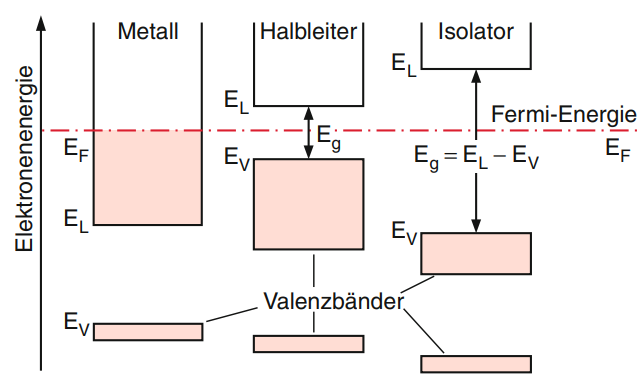
\includegraphics[width=0.7\textwidth]{figure/halbleiter.png}
    \caption{Übersicht des Bändermodells von Halbleitern. Dargestellt sind die Unterschiede zwischen Metallen, Halbleitern und Isolatoren \cite{demtroder}.}
    \label{fig:halbleiter}
\end{figure}
Die Halbleiter können dotiert werden, dabei werden Fremdatome in den Kristall eingebaut.
Diese Fremdatome besitzen mehr oder weniger freie Elektronen, wodurch entweder die Anzahl freier Elektronen oder die Anzahl Löcher erhöht werden kann.
Im Fall der n-Dotierung wird ein Atom mit mehr freien Elektronen eingebaut, wodurch unterhalb des Leitungsbandes sogenannte Donatorniveaus entstehen.
Für diese Niveaus ist die Bandlücke deutlich kleiner, wodurch weniger Energie aufgewendet werden muss.

\subsection{Faraday-Effekt}
\label{ssec:faraday}

Der Faraday-Effekt beschreibt die Drehung von linear polarisiertem Licht um einen bestimmten Winkel innerhalb eines doppelbrechenden Materials parallel zu einem B-Feld.
Das linear polarisierte Licht kann in einen links- und rechts-zirkularen Teil zerlegt werden. 
Beide Bestandteile des Lichts besitzen im Medium verschiedene Ausbreitungsgeschwindigkeiten und die resultierende lineare Polarisation dreht sich.
Der Winkel um den sich das Licht dreht ist gegeben durch
\begin{equation}
    \theta = \frac{e^3 \lambda^2 N B L}{8 \pi^2 \epsilon_0 c^3 {m^*}^2 n}.
    \label{eqn:theta}
\end{equation}
Dabei ist $B$ die Stärke des Magnetfeldes, $m^*$ die effektive Masse der Elektronen, $N$ die Donatorkonzentration, $n$ der Brechungsindex und $L$ die Probendicke.
Der Faraday-Effekt ist schematisch in \autoref{fig:doppel} dargestellt.
\begin{figure}
    \centering
    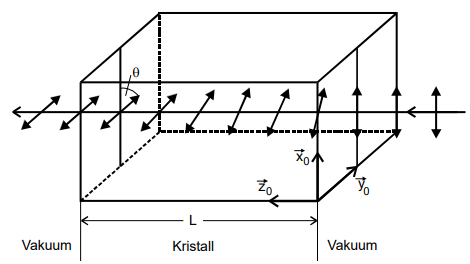
\includegraphics[width=0.7\textwidth]{figure/doppelbrechung.png}
    \caption{Schematische Darstellung der Drehung des linear polarisierten Lichts \cite{anleitung}.}
    \label{fig:doppel}
\end{figure}